\section{Hyperparameters optimization}\label{sec:activityhyperopt}

The hyperparameters optimization has been conducted in the same way done in
\chref{sec:mlphyperopt}. In particular, the stage used to do the optimization
with \code{bayesopt} (the \code{hyperoptmlp} stage) has been copy-pasted in
a new stage named \code{hyperoptmlp\_act}\footnote{This is a general approach.
Whenever you see a file (stage or script) named \code{<something>\_act}, this
is the same \code{<something>} stage/script adapted for the MLP developed in
this chapter.} and adapted to be used with \code{patternet}.

Hyperparameters to be optimized are the following:
\begin{itemize}
\item The architecture of the network (the number of hidden layers and the
	number of hidden units in each layer);
\item The training algorithm;
\item The hyperparameters of the training algorithm.
\end{itemize}

\subsection{Training algorithm selection}\label{subsec:activityhyperopt}

Script \code{mlphyperopt\_act.m} tries to find the optimal training algorithm
for the network. The script is just the adaptation of the script used in
\secref{subsec:mlphyperopt}.

The script uses the \code{pretrainingpipeline} function to build the same two
pipelines used in the previous chapter. Output of \code{buildfeaturematrix}
stages of these 2 pipelines is then merged together in a single feature matrix
by the \code{mergefeaturematrix} stage. This way, the feature extracted in
\chref{ch:ecg} can be used here without the need to re-extract them again.

The output of the \code{mergefeaturematrix} stage is then passed muliple times
to the \code{trainmlp\_act} stage, which performs the training of the network.

The list of training algorithm tested is the same of
\secref{subsec:mlphyperopt}, with the exception of the \code{trainlm} and
\code{trainbr} algorithms, which have been removed since they do not support
the use of the performance function \code{crossentropy}.

Data has been partitioned as follows:
\begin{itemize}
\item Training set: \(70\%\) (\(4200\) samples).
\item Validation set: \(15\%\) (\(900\) samples).
\item Test set: \(15\%\) (\(900\) samples).
\end{itemize}
A difference with the partitioning used in the previous chapter, is that this
time stratification has been used in order to get 3 sets with the same number
of samples for each class. This is done by the function
\code{stratifieddividerand}.

Results are shown in \lstref{lst:activityhyperopt}. The scaled conjugate
gradient backpropagation algorithm (\code{trainscg}) is the one which produced
the best results.

\lstinputlisting[language={}, label={lst:activityhyperopt}, caption={Result of
the execution of the \texttt{mlphyperopt\_act.m}
script.}]{activityhyperopt.txt}

\subsection{Bayesian optimization of the network's architecture and training
algorithm's hyperparameters}\label{subsec:activitybayesopt}

Just like has been done in \secref{subsec:mlpbayesopt}, here, using the script
\code{mlpbayesopt\_act.m}, I've executed \code{bayesopt} with \standout{5-fold
cross-validation} to optimize the following parameters:

\begin{description}
\item[hiddenLayers] The number of hidden layers. Range:
	\(\interval{1}{3}\).
\item[hiddenUnits1] The number of hidden neurons in the first layer. Range:
	\(\interval{40}{180}\).
\item[hiddenUnits2] The number of hidden neurons in the second layer. Range:
	\(\interval{0}{65}\).
\item[hiddenUnits3] The number of hidden neurons in the third layer. Range:
	\(\interval{0}{20}\).
\item[\(\mu\) (\code{mu})] The Marquardt adjustement parameter. Range:
	\(\interval{0.001}{0.01}\).
\item[\(\sigma\) (\code{sigma})] The parameter that determines change in weight
	for second derivative approximation. Range:
	\(\interval{\num{1.0e-5}}{\num{1.0e-4}}\).
\item[\(\lambda\) (\code{lambda})] The parameter used for regulating the
	indefiniteness of the Hessian. Range:
	\(\interval{\num{1.0e-7}}{\num{1.0e-6}}\).
\end{description}

Since I'm going to optimize more parameters, the number of epochs evaluated by
\code{bayesopt} has been increased from 100 to 500 epochs.
\tableref{table:activitybayesopt} shows the best parameters selected for the
network. \figref{fig:activityarch} shows the chosen architecture in a graphical
representation.

\begin{table}[hbtp]
	\centering
	\begin{tabular}{|l|c|}
		\toprule
		Parameter & Value \\
		\midrule
		hiddenLayers & 2 \\
		hiddenUnits1 & 165 \\
		hiddenUnits2 & 31 \\
		hiddenUnits3 & 0 \\
		\(\mu\) (\code{mu}) & \num{0.00503782845709468} \\
		\(\sigma\) (\code{sigma}) & \num{5.24912243184705e-5} \\
		\(\lambda\) (\code{lambda}) & \num{2.39459690552712e-7} \\
		\bottomrule
	\end{tabular}
	\caption{Best parameters and architecture selected by \code{bayesopt}
	for the activity recognition network.}\label{table:activitybayesopt}
\end{table}

\begin{figure}[htbp]
	\centering
	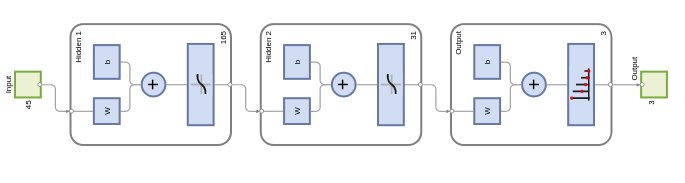
\includegraphics[width=\linewidth]{activityarch}
	\caption{The chosen architecture for the activity recognition network.}
	\label{fig:activityarch}
\end{figure}
